\section{Logic of Events}
\label{sec_logic}

% %% einleitung %%
% In diesem Kapitel wird die Eventlogik~\cite{bickford2003logic} nach Bickford und
% Constable vorgestellt. Dazu werden vorher die benötigten grundlegenden Logiken
% und Theorien eingeführt. Zuerst wird kurz die Aussagenlogik erklärt und die
% darauf aufbauende Prädikatenlogik, welche grundlegend sind um ein Verständnis
% für die späteren Formeln zu liefern. Danach wird auf die intuitionistische
% Interpretationsweise und konstruktive Logik eingegangen. Als weitere Grundlagen
% werden ein Einführung in die Typentheorie und Automatentheorie gegeben, soweit
% dass für das weitere Verständnis der Eventlogik notwendig ist.

% \subsection{Grundlegende Logiken}
% Die Mathematische Logik ist eine mathematische Theorie in der andere
% mathematische Modell mit Hilfe "`naiver Logik"' formalisiert werden können.
% Die mathematische Logik bietet damit eine Metasprache zur Untersuchung anderer
% mathematischer Modelle.~\cite{heinemann2013logik}

% \paragraph{Aussagenlogik}
% Sie ist die älteste Logik und benutzt aus Grundelement Aussagen (Atome,
% Literale) zur Formalisierung. Aussagen sind können entweder \textbf{wahr}
% oder \textbf{falsch} sein. \textbf{Terme} sind aussagenlogische Formeln
% bei der einzelne Aussagen über \textbf{Junktoren} verbunden sind.~\cite{heinemann2013logik}

% \begin{defi}
%   Sei $\Sigma_A := \{V,(,),\neg,\vee,\wedge,\Rightarrow,\Leftrightarrow,\bot,\top\}$ das Alphabet der Aussagenlogik, wobei $\top$ für
% wahr, $\bot$ für falsch, $\neg$ für die Negation, $\vee$ für die Disjunktion, $\wedge$ für die
% Konjunktion , $\Rightarrow$ für die Implikation und $\Leftrightarrow$ für die Äquivalenz steht.
% \begin{itemize}
% \item $V:=\{p_0,p_1,..\}$  ist die Menge der Variablen oder Symbole
% \item $T\subseteq W(\Sigma)$  ist die Menge der Terme die über $\Sigma$ gebildet werden können
% \end{itemize}
% \end{defi}

% \begin{defi}
%   Ein Term ist definiert als
%   \begin{itemize}
%   \item $V\subseteq T$
%   \item $\{\top,\bot\}\subseteq T$
%   \item $\{\neg\alpha,(\alpha\vee\beta),(\alpha\wedge\beta),(\alpha\Rightarrow\beta),(\alpha\Leftrightarrow\beta)\}\subseteq T$, falls $\alpha,\beta\in T$
%   \end{itemize}
% \end{defi}

% Als Beispiel kann der Satz "`Wenn X keine Zahl ist, dann kommt danach ein
% Buchstabe."' in die Formel
% \[
%   \neg x_{Z} \Rightarrow x_{B}
% \]
% übersetzt werden.

% Terme können ausgewertet werden und ihnen Wahrheitswerte zugeordnet werden.
% Dazu werden Interpretationen für die vorkommenden Variablen angegeben.

% \begin{defi}
%   Die Interpretation ist eine mögliche Belegung für einen Term $t$ und
%   wird als $I:L(t)\rightarrow \{wahr,falsch\} \Leftrightarrow t^I$ geschrieben.
%   Eine Interpretation die eine Formel $t^I$ wahr werden lässt, \textbf{erfüllt}
%   diese Formel.
% \end{defi}

% Eine besondere Art eines Terms ist die \texttt{Tautologie} bei der jegliche
% Interpretion wahr wird. Eine Tautologie ist eine allgemeingültige Ausage.

% \begin{defi}
%   Axiome sind Terme einer Logik, die ohne Angabe von Rechtfertigungen als wahr angenommen
%   werden. Axiome werden zumeist als semantische Tautologien gewählt, wobei sie
%   syntaktisch gesehen formale Terme ohne besondere Bedeutung sind.
% \end{defi}

% Aus den Tautologien und Axiomen einer Logik können weitere Terme abgeleitet
% werden. Zur Ableitung weiterer gültiger Terme aus einer Logik werden
% Schlussregeln oder Inferenzregel benutzt. Ein System aus Inferenzregeln zum
% Schließen über Tautologien und möglicherweise Axiomen einer Logik wird Kalkül genannt.

% \begin{defi}
%   Sei $\Gamma$ eine endliche Menge von Termen einer Logik und $C$ ein Term der Logik.
%   Dann ist $C$ aus $\Gamma$ ableitbar, wenn es eine Folge von Inferenzregeln
%   $r_0,...,r_n$ und Termen $C_0,...,C_n$ gibt, so dass $C_n = C$ und
%   $\Gamma_0\vdash_{r_0}C_0 ... \Gamma_n\vdash_{r_n}C_n$ wobei $\Gamma_i$ die Menge aller Axiome, Terme
%   aus $\Gamma$ und bisher abgeleiteten Terme enthält.
% \end{defi}

% \subsection{Prädikatenlogik}
% Die Prädikatenlogik stellt eine Erweiterung der Aussagenlogik dar.
% Bei der Aussagenlogik werden atomare Aussagen oder Literale mit konkreten
% Wahrheitswerten belegt. In der Aussagenlogik können nicht alle Aussagen
% mit Wahrheitswerten belegt werden, da manche Belegungen von der inneren
% Struktur der Aussage abhängen. Zum Beispiel der Satz "`x ist eine Primzahl"'
% hängt von einer konkreten Belegung $x$ ab und ist in der Aussagenlogik kein
% valides Literal. Diese Abhängigkeit wird durch Prädikate ausgedrückt.~\cite{heinemann2013logik}

% \begin{defi}
%   Das Alphabet der Prädikatenlogik ist $\Sigma_P := \{\exists,\forall,F,V,P\} \cup \Sigma_A$, wobei
%   $\exists$ als \texttt{es existiert} und $\forall$ als \texttt{für alle gilt} gelesen wird.
%   $V$ ist die Menge der Variablen, $P$ ist die Menge der Prädikate und $F$ ist die Menge der
%   Funktionen in der Prädikatenlogik.
% \end{defi}

% \begin{defi}
%   Ein \textbf{Prädikat} der Stelligkeit \textbf{n} ordnet einem Variablentupel
%   $(x_1,...,x_n)$ der Mengen $M_1,...,M_n$ Wahrheitswerte zu, daraus folgt
%   $P(x_1,...,x_n) \rightarrow \{wahr, falsch\}$ wobei $x_i\in M_i$ für $i\in \{1,...,n\}$.
% \end{defi}
% Ein Prädikat, dass ein Tupel erfüllt, ordnet dem Tupel den Wahrheitswert wahr zu.

% \begin{defi}
%   Sei $\mathbb{F}=\Cup^{\infty}_{i=0}\mathbb{F}^i$ für jedes $0\le i$ ein Alphabet von
%   i-stelligen Funktionssymbolen und $\mathbb{V}$ ein Alphabet von Variablen,
%   dann sind Terme der Prädikatenlogik definiert als:
%   \begin{itemize}
%   \item $x\in\mathbb{V}$ ist ein Term
%   \item $f\in\mathbb{F}^0$ ist ein 0-stelliges Funktionssymbole und eine Term der
%     eine Konstante ist
%   \item $t_1,...,t_n$ sind Terme und $f\in\mathbb{F}^n$ ein n-stelliges
%     Funktionssymbol, dann ist $f(t_1,...,t_n)$ ein Term
%   \end{itemize}
% \end{defi}~\cite{kreitz1994automatisierte}

% Zur Darstellung von konkreten Sprachen müssen Bezeichner aus der Menge aller
% Bezeichner aussortiert werden. Damit wird eine konkrete Sprache mit einem Typ
% versehen.
% \begin{defi}
%   Ein Typ $T$ ist eine Paar $(I,J)$ mit $I\subseteq P$ und $J\subseteq F$.
% \end{defi}~\cite{heinemann2013logik}

% Damit ist es möglich die Formeln der Prädikatenlogik zu definieren.

% \begin{defi}
%   Sei $\mathbb{P}^i$ mit $0\le i$ ein i-stelliges Prädikatenalphabet,
%   $\mathbb{P}=\Cup^{\infty}_{i=0}\mathbb{P}^i$ und $\mathbb{T}$ ein Alphabet von Typen,
%   dann ist eine Formel der Prädikatenlogik definiert als:
%   \begin{itemize}
%   \item $P\in\mathbb{P}^0$ ist ein 0-stelliges Prädikatensymbol und damit P eine
%     atomare Formel oder Aussagenvariable
%   \item $t_1$ und $t_2$ sind Terme, dann ist $t_1 = t_2$ eine atomare Formel,
%     die gewöhnliche Gleichheit ausdrückt.
%   \item $t_1,...,t_n$ mit $n\geq1$ sind Terme und $P\in\mathbb{P}^n$ ein n-stelliges
%     Prädikatensymbol, dann ist $P(t_1,...,t_n)$ eine atomare Formel
%   \item $A,B$ sind Formel, $x\in\mathbb{V}$ eine Variable und $T\in\mathbb{T}$ ein
%     Typenbezeichner, dann sind $\neg A$, $A\vee B$, $A\wedge B$, $A\Rightarrow B$, $\forall x:T.A$, $\exists
%     x:T.A$ und $(A)$ Formeln
%   \end{itemize}
% \end{defi}~\cite{kreitz1994automatisierte}

% Eine Interpretation für eine prädikatenlogische Formel ist lediglich eine
% Erweiterung der aussagenlogischen Interpretation, um die Belegungen von
% n-stelligen Prädikat- und Funktionssymbolen.~\cite{heinemann2013logik}

% \paragraph{Bindung}
% Zur besseren Lesbarkeit werden Klammer für die Bindungsstärke von Junktoren
% zumeist weggelassen. Dadurch ergibt sich die implizite Bindungsreihenfolge:
% $\neg,\wedge,\vee,\Rightarrow,\exists,\forall$.~\cite{kreitz1994automatisierte}

% Die Prädikatenlogik stellt das Grundgerüst, auf dessen Basis die später
% vorgestellte Eventlogik steht. Sie ermöglicht die Formalisierung von natürlichen
% Aussagen und Theorien, sowie die Überprüfung derer Gültigkeit.

% \subsection{intuitionistische Logik}
% Bisher wurden die Logik mit ihrer klassischen Interpretation vorgestellt.
% Dabei wird angenommen das eine Aussage entweder wahr oder falsch ist.
% Anders ausgedrückt kann ein mathematische Objekt entweder existieren oder
% nicht. Beweise auf Grundlage dieser Interpretationsansicht erfordern keine
% konstruktive Herleitung, wie ein solches Objekt zu modellieren ist.
% Das Gesetz vom ausgesschlossenen Dritten $A\vee\neg A$, die doppelte Negation $\neg\neg A\Rightarrow
% A$, Wiederspruchsbeweise und "`ex falso sequitur quodlibet"' gehören zu den
% problematischen Beweisansätzen, die keine intrinsische Rechtfertigung
% benötigen.~\cite{sep-logic-intuitionistic}

% Brouwer hat 1908 festegestellt, dass $A\vee\neg A$ angewendet auf unendliche
% abzählbare Mengen zu Problemen führt. Ein Beispiel dafür ist die Goldbach
% Vermutung, die annimmt, dass jede Zahl $> 2$ als Summe zweier Primzahlen
% geschrieben werden kann. Diese Aussage ist bis heute unbewiesen. Die klassische
% Logik umschifft solche Probleme in dem sie annimmt, dass weder die Aussage, noch
% ihr Gegenteil gleichzeitig falsch sein kann, ohne eine konstruktive
% Rechtfertigung dafür zu liefern. Dabei ist es für den geneeigten Leser
% einsichtig, dass keine einfache Funktion, nach der Church-Turing These,
% gefunden werden kann, die in absehbarer Zeit eine Lösung oder Beweis der
% Aussage liefert.~\cite{sep-logic-intuitionistic, sep-mathematics-constructive}

% Der Intuitionismus und die konstruktive Mathematik lehnen diese Art der
% Beweisführung und die Allgemeingültigkeit der vorher erwähnten Gesetze ab.
% Dabei werden verschiedene logische Operationen anders interpretiert.
% Zum Beispiel wird von der Disjunktion $A\vee B$ verlangt, dass sie angeben kann
% welcher Teil beweisbar ist und einen entsprechenden Beweis (Evidenz)
% dafür liefert.~\cite{kreitz1994automatisierte}

% \begin{defi}
%   Die intuitionistische Interpretation der Prädikatenlogik setzt sich aus
%   Evidenzen zusammen die in den Teilaussagen gefordert sind.
%   \begin{itemize}
%   \item Jedes Literal $q$ besitzt eine Evidenz $e$
%   \item Um $P\vee Q$ zu beweisen, ist entweder die Evidenz für $P$ oder $Q$
%     notwendig
%   \item Um $P\wedge Q$ zu beweisen, ist die Evidenz von $P$ und $Q$ notwendig
%   \item Um $P\Rightarrow Q$ zu beweisen, muss ein Algorithmus angegeben werden, der jede
%     Evidenz für $P$ in eine Evidenz für $Q$ umwandelt
%   \item Um $\neg P$ zu beweisen, muss gezeigt werden, dass es keinen Beweis gibt
%   \item Um $\exists x:T.P(x)$ zu beweisen, muss ein Objekt vom Typ $T$ konstruiert
%     und gezeigt werden, dass $P$ hält.
%   \item Um $\forall x\in T.P(x)$ muss gezeigt werden, dass jedes Objekt $x$ den Typ $T$
%     hat und darunter $P$ beweisbar ist.
%   \end{itemize}
% \end{defi}~\cite{sep-mathematics-constructive}

% Die intuitionistische Logik ermöglicht damit Kalküle zu entwickeln auf
% deren Grundlage beweisbare logische Schlüsse erzeu
% gt werden können.
% Damit kann sie als eine höhere Programmiersprache angesehen werden.
% Beweise die konstruiert werden können mit Hilfe der Curry-Howard Isomorphie
% in Typsysteme überführt werden und ausprogrammiert werden.~\cite{constable1970constructive}

% \subsection{Martin-Löf Typentheorie}
% Verschiedene Kalküle wurden für die Prädikatenlogik entwickelt.
% In dieser Arbeit wird nur auf die Typentheorie von Per Martin Löf eingegangen,
% da sie die Grundlage für den interaktiven Theorembeweiser
% NuPRL\footnote{\url{http://www.nuprl.org/Intro/intro.html}} ist. In NuPRL ist
% die später vorgestellte Eventlogik formalisiert und bewiesen worden.

%% eventlogik %%
% \subsection{Eventlogik}

% Mark Bickford und Richard L. Constable haben in verschiedenen
% Papern~\cite{bickford2003logic, bickford2005causal, bickford2009component} eine Logik zur Beschreibung
% von Ereignissen in verteilten Systemen vorgestellt. Die Eventlogik ist so
% aufgebaut, dass eine breite Menge von Systemen beschrieben werden kann, auch
% außerhalb des eigentlichen Anwendungsgebietes des verteilten Rechnes
% (Distributed Computing).  Die Logik ist auf der
% intuitionistischen Logik aufgebaut und folgt dem ``correct-by-construction''
% Ansatz. Bei diesem Ansatz werden aus Beweisen für Formeln korrekte Implementierungen für
% diese gewonnen.~\cite{bates1985proofs}

% Dafür wird eine abstrakte Spezifikationssprache eingeführt welche durch
% ein Berechenbarkeitsmodell repräsentiert wird.
% Schlussfolgerungen in diesem Modell werden durch Inferenzregeln dargestellt und
% ermöglichen es, wenn eine Spezifikation erfüllbar ist, ein ausführbares
% verteiltes System aus dem Modell zu extrahieren.~\cite{bickford2005causal}

% \paragraph{typentheoretische Vorbetrachtung}
% Um der Eventlogik eine mathematische Struktur zu geben, werden ihre
% Elemente mit diskreten Typen beschrieben, d.h. dass ihre die Gleichheit
% entscheidbar ist und sie voneinander disjunkt sind.

% \begin{defi}
%   $\mathbb{D}$ ist der Typ der alle diskreten Typen enthält $T\in\mathbb{D}$ mit $\{T:Type|\forall x,y : T.x = x\ in\ T \vee\neg (x = y\ in\
%   T)\}$.
% \end{defi}

% \subsubsection{Events}
% Events bilden die Grundbausteine der Eventlogik.
% Sie stellen Aktionen dar die in Raum und Zeit passieren und
% werden ohne Zeitdauer definiert.
% Die Zeitdauer eines Events würde sich auf die physische Zeit der
% Umsetzung beziehen und wurde der zur Vereinfachung
% wegabstrahiert.~\cite{bickford2005causal}


% \begin{defi}
%   Ein Event $e$ ist die atomare Einheit und kausal geordnet, d.h.
%   $e< e'$ wenn $e$ zeitlich vor $e''$ passiert ist.
% \end{defi}

% \begin{defi}
%   Events $e\in E$ sind in einem Eventraum strukturiert. Dieser besteht
%   aus einzelnen $loci$ oder Entitäten an denen Events passieren.
% \end{defi}

% Der Eventraum ist dynamisch aufgebaut, so dass über die Zeit neue Entitäten
% hinzugefügt oder entfernt werden können. Damit die Entitäten im Raum
% unterschieden werden können besitzen sie beobachtbare Eigenschaften, wie zum
% Beispiel Koordinaten oder eine ID. Zur theoretischen Betrachtung reicht es aus,
% wenn Entitäten durch einen diskreten Typen und eine ID unterschieden werden können.~\cite{bickford2005causal}

% \begin{defi}
%   Jede Entität ist mit jeder anderen Entität über mindestens
%   einen Kommunikationsweg ($link$) verbunden.
% \end{defi}

% Für die $links$ wird das nicht-byzantinische Fehlermodell angenommen,
% wobei die Verbindungen unzuverlässig sind, aber die Nachrichten nicht
% verfälschen. Ein Event kann zur Kommunikation Nachrichten über einen
% $link$ versenden.


% Da Events an Entitäten gebunden sind, können sie kausal strukturiert werden.
% Damit können Events folgendermaßen formalisiert werden.
% \begin{gather*}
%   \textbf{E:}\mathbb{D}\notag\\
%   \textbf{Loc:}\mathbb{D}\\
%   \textbf{pred?:} E\rightarrow (E+Loc)\\
%   \textbf{sender?:} E\rightarrow (E+Unit)
% \end{gather*}

% E ist ein Event und Loc eine Entität. Die Funktion $pred?$ gibt entweder das
% vorherige Event an der Entität zurück oder die Entität, wenn es das erste Event
% war. Die Funktion $sender?$ gibt des Event $e'$ zurück, dass das Event $e$
% ausgelöst hat oder den leeren Typ.~\cite{bickford2005causal}

% Mit diesen Grundannahmen können die Funktionen $first?$, die bestimmt ob
% ein Event das Erste ist, dass bei einer Entität passiert und $recv?$,
% dass bestimmt ob ein Event ein Empfangsevent ist, definiert werden.

% \begin{gather*}
%   \textbf{first?:}E\rightarrow (E\rightarrow (E+Loc))\rightarrow B\\
%   first?(e,pred?) = if\ is\_left(pred?(e))\ then\ true\ else\ false\\
%   \textbf{recv?:}E\rightarrow (E\rightarrow (E+Unit))\rightarrow B\\
%   recv?(e,sender?) = if\ is\_left(sender?(e))\ then\ true\ else\ false\\
% \end{gather*}

% Mit Hilfe dieser Funktionen lässt sich die Eingangserwähnte kausale Ordnung auf Events
% $e < e'$ definieren als:
% \[
%   pred!(e,e') == (\neg first(e')\Rightarrow e = pred?(e')) \vee e = sender(e')
% \]
% $pred!$ bildet eine transitive Hülle und stellt damit eine wohlgeordnete
% entscheidbare Ordnung der Form $e < e'$ dar. Als letztes fehlen noch
% drei Grundaxiome für den geordneten Eventraum.~\cite{bickford2005causal}

% \begin{axiom}
%   Wenn ein Event $e$ ein Signal sendet, dann gibt es ein Event $e'$, so dass für
%   jedes Event $e''$ gilt, $e'' = e'$ oder $e'' < e'$.\\
%   \[
%     \forall e:E \exists e':E. \forall e'':E . (recv?(e'') \& sender?(e'')=e)\Rightarrow (e' = e' \vee e'' < e)
%   \]
% \end{axiom}

% \begin{axiom}
%   Die Funktion $pred?$ ist injektiv.
%   \[
%     \forall e,e':E.loc(e) = loc(e')\Rightarrow pred?(e) = pred?(e')\Rightarrow e=e'
%   \]
% \end{axiom}

% \begin{axiom}
%   Die Funktion $pred!$ bildet eine starke wohlfundierte Ordnung.
%   \[
%     \exists f:E\rightarrow \mathbb{N}.\forall e,e':E.pred!(e,e')\rightarrow f(e)<f(e')
%   \]
% \end{axiom}

% \begin{defi}
%   Die folgenden Notationen werden als Abkürzung verwendet, um Events die an einem
%   Ort stattfinden zu quantifizieren.
%   \[
%     \forall e@i.P == \forall e:E.(loc(e) = i\Rightarrow P)
%   \]
%   \[
%     \exists e@i.P == \exists e:E.(loc(e) = i\Rightarrow P)
%   \]
% \end{defi}

% Abbildung~\ref{fig:sequence} zeigt ein einfaches Beispiel über einen Eventraum,
% der sich mit der bisherigen Theorie spezifizieren lässt. Dort wird eine 1:1
% Kommunikation zwischen zwei Entitäten dargestellt. Jede Nachricht von S wird mit
% einer Antwort von R quitiert, bevor eine neue Nachricht von S bei R eintrifft.
% Diese Modell kann forlgendermaßen formalisiert werden:~\cite{bickford2005causal}

% \begin{gather*}
%   \forall s@S.\exists r'@R.s=sender?(r')\\
%   \exists r@S.(s<r\&\exists s''@R.(r'\leq s''\& sender?(r) == s''))\\
% %%  \forall x@S.s<x<r\Rightarrow x wird nicht an R gesendet\\
%   \forall x@S.s<x<r\Rightarrow \neg\exists x'@R.(x=sender?(x'))
% \end{gather*}

% Als nächstes werden Events erweitert um Werte und unterschieden nach
% $internen$ und $externen$ Events. Bei einem $externes$ Event sendet ein Sender
% einer Nachricht über einen $link$ zu einem Empfänger. $Interne$ Events können
% ebenfalls Werte übergeben und können durch $guards$ limitiert werden.~\cite{bickford2005causal}

% \begin{defi}
%   Der Typ eines Events ist:
%   \[
%     kind == (Act+Top)
%   \]
%   \[
%     kind: E\rightarrow (Act+Top)
%   \]
%   Dabei ist Act ein diskreter Typ um unterschiedle interne Events, zu
%   unterscheiden und Top der Wert eines externen Events.
% \end{defi}

% Eine Darstellungsform von Interaktionen und Eventräumen sind Sequenzdiagramme
% mit Nachrichten, wie in Abb.~\ref{fig:sequence} dargestellt.
% % EValues vllt vertiefen, funktionalität beschreiben?

% \begin{defi}
%   Eine Entität kann einen Zustand haben der durch eine endliche Folge
%   von Änderungen dargestellt werden kann. $s'=f(s,v)$, wobei
%   $v'$ der Folgezustand und $v$ der Wert eines Events ist.
% \end{defi}

% Die Eventlogik nach Bickford und Constable baut auf der intuitionistischen Logik
% auf. Sie verfolgt den ``correct-by-construction'' Ansatz, nach dem ein
% funktionales Programm aus einem konstruktiven Beweis extrahiert werden kann.
% Die Beweise haben die Grundform $\forall x:A.\exists : B.spec(x,y)$. Der konstruktive Beweis
% liefert einen Extraktterm, der eine Realisierung des Beweises darstellt.
% Da die Eventlogik die konstruktive Typentheorie benutzt sind alle
% beweisbaren logischen Aussagen auch programmierbar, in dem Sinne, dass sie einen
% Extraktterm besitzen der die Spezifikation erfüllt.~\cite{bickford2003logic}


% TODO
% Aussagenlogik +
% Prädikatenlogik 1. Ordnung +
% intuitionistische Logik +
% Martin Löf Typentheorie
% Automatentheorie NEA?
% Eventlogik +?
% RAFT Zensusprotokoll



This chapter introduces the logical and programmatic foundations needed for this
thesis. To achive this, it is split into two parts. The first part introduces
the reader with the Logic of Events which is the theoretical foundation for the
Velisarios framework. The second part provides a practical introduction to
the basics of COQ and programming with Velisarios.

\subsection{Logic}

The Logic of Events was introduced by Bickford and
Constable~\cite{bickford2003logic} to describe parallel systems which
consists out of nodes and events happening between them. To follow
the explenation a brief overview about propositional logic, predicativ logic,
constructive logic and type theorie is presented. It is assumed that the reader
is already familiar with the basic logical systems.

\paragraph{Propositional Logic}
The oldest known logic uses atoms or a set of primitive symbols and logical
connective or a set of operator symbols to formalize
terms or propositions about the world. Statements in classical logic can be either
\textbf{true} or \textbf{false}. The table~\ref{tab:proplogic} provides
a short description for the logical connectives and their meaning.~\cite{heinemann2013logik}

\begin{table}[h]
  \centering
  \begin{tabular}{c|c|l}
    Symbols & Example & Description\\\hline
    $A,B,C,...$ & $P, Q$ & Atoms used in propositions.\\
    $\neg$ & $\neg P$ & Negation of some atom or proposition.\\
    $\vee$ & $P \vee Q$ & The disjuction of two propositions.\\
    $\wedge$ & $P \wedge Q$ & The conjunction of two propositions.\\
    $\Rightarrow$ & $P \Rightarrow Q$ & The implication of two propositions.\\
    $\Leftrightarrow$ & $P \Leftrightarrow Q$ & The equivalence composed of two propositions.\\
  \end{tabular}
  \caption{Overview of propositional logic symbols}
  \label{tab:proplogic}
\end{table}

To make sense out these defined terms these need to be evaluated. To do so,
the atoms are assigned to thruth values which is called the \textit{interpretation}.~\cite{tuschik1994mathematische}

\begin{defi}
  More formal, an interpreation is a sample assigned for a term $t$ with
  $I:L(t)\rightarrow \{true,false\} \leftrightarrow t^I$. Interpretation which suffices the term
  $t^I$ are called a \textit{model}.
\end{defi}

The most defined formal systems using terms which are taken as truth without
proof or justification. These terms are called \textit{axioms}. These are syntactically
without meaning but semantically always the truth.~\cite{tuschik1994mathematische}

To gather new knowledge out of axioms, terms and atoms a way to conclude
new terms is needed. This can be done by adding \textit{inference rules} to
the system. These rules derive new terms oder conclusions out of a given
set of propositions. Such a formal system is called \textit{logical calculus}.~\cite{tuschik1994mathematische}

\paragraph{Predicate logic}
The predicate logic is an extension of the propositional logic.
For instance, the statement ``x is a prime number'' can't be described
in propositional logic since the thruth value depends on the structure of $x$.
The predicate logic adds \textit{quantifiers} and \textit{predicates} to the
system to describe atoms with variable structures.~\cite{heinemann2013logik}

\begin{table}[h]
  \centering
  \begin{tabular}{c|c|l}
    Symbols & Example & Description\\\hline
    $a,b,...$ & $x,y$ & The set of variables $\mathcal{V}$.\\
    $P_0^n,Q_1^n,...$ & $P(x_1,...,x_n)$ & The set of predicates $\mathcal{P}$ with arity $n$
                                          which evaluates to $\{true,false\}$\\
    $f_0^n,g_1^n,...$ & $f(t_1,...,t_2)$ & The set of formulas $\mathcal{F}$with arity $n$\\
    $\forall$ & $\forall x.P(f(x))$ & The quantifier means that for all possible allocations the term holds.\\
    $\exists$ & $\exists x.P(x)\Rightarrow Q$ & The quantifier means that for some allocations the term holds.\\
    $=$ & $x = y$ & The equality is added as connective to the alphabet.\\
  \end{tabular}
  \caption{Overview of predicate logic symbols}
  \label{tab:predlogic}
\end{table}

The table\,\ref{tab:predlogic} presents the extension made by the predicate logic.
Since the predicate logic is mathematically used to describe objects,
structure and their relations it is useful to define such structures.~\cite{heinemann2013logik}

\begin{defi}
  The type $T$ is a pair of $(I,J)$ where $I\subseteq P$ and $J\subseteq F$.
  Therefore, predicates are relations between objects of the underlying
  structure.
\end{defi}

The interpretation is similar to propositional logic execept it is
extended with $n$-artity predicate- and functionsymbols.~\cite{heinemann2013logik}

\paragraph{Intuitionistic logic}
The propositional and predicate logic are presented with the classical
interpretation. The classical interpretation assumes that every statement
is either $true$ or $false$ or more elaborated a mathematical object either
exists or not. Therfore, proofs with classical interpretation don't care
about how such an object is constructed. For example the law of double
negation eliminitation  $\neg\neg A\Rightarrow A$ or the Aristotelian law of excluded
middle $A \vee \neg A$, are such problematic laws. These laws don't provide
intrinsic justification, in the way that they don't construct an object
of that type or prove that it ``exists''.~\cite{sep-logic-intuitionistic, kreitz1994automatisierte}

This problem was found by Brouwer in 1908. He observed that $A \vee \neg A$
applied on infinite sets lead to problems. An example is the Goldbach
conjencture which assumes that every number $> 2$ can be expressed out of
two prime numbers. The classical logic uses a wider interpretation
the law of excluded middle to get around this problem. It assumes
that one of the cases must be true and none of them is not an option.
As a side-effect such an interpretation rejects to be generally
appliable to mathematical computational models.~\cite{sep-logic-intuitionistic, sep-mathematics-constructive}

The \textit{intuitionism} is a mathematical direction of thinking which
rejects the line of argument and universality of the law of excluded middle
and other laws of that type. For this reason, the intuitionism demands
that mathematical statements are seen as constructive statements.
For instance, the exists quantifiers $\exists x.A$ is re-interpeted in a way
that a real object can be given and is not only a theoretical one.
Logical connective are also re-intepreted that they give a way
of constructing a proof with real objects and at every time one can
say which way the proof uses. One can see from the \textit{evidence}
of some proof with the disjunction $A\vee B$ which part of the disjunction
leads to a correct proof.~\cite{kreitz1994automatisierte}

\begin{table}[h]
  \centering
  \begin{tabular}{c|l}
    Symbols &  Description\\\hline
    $q$ & Every literal $q$ has some evidence $e$.\\
    $P\vee Q$ & The proof demands either an evidence for $P$ or $Q$ and mark it.\\
    $P\wedge Q$ & The proof demands an evidence for booth $P$ and $Q$.\\
    $P\Rightarrow Q$ & The proof demands an effective algorithm which\\
           & converts every proof for $P$ into one for $Q$.\\
    $\neg P$ & To proof the abscence one must show that there is no proof for it.\\
    $\exists x:T.P(x)$ & The proof needs an constructed object of type $T$ which holds for $P$.\\
    $\forall x:T.P(x)$ & The proofs demands that for every object $x$ out of the type $T$\\
                 &  $P$ there is an effective algorithm which computes a proof.
  \end{tabular}
  \caption{Intuitionistic interpretation of the typed predicate logic~\cite{sep-mathematics-constructive}}
  \label{tab:intsymbols}
\end{table}

the table~\ref{tab:intsymbols} show the intuitionistic interpretation for the logical
symbols in typed predicate logic. As an application example, proofs about
programs can only be done \textit{constructive} since a proof of contradiction
says nothing about how to construct such a program or if the program
fulfills some property.~\cite{kreitz1994automatisierte}
Therefore, within the rest of this theses logical
statements uses the intuitionistic logical interpretation.

\paragraph{proofs-as-program}
Taken the intuitionistic interpretation into computer science then for
mathematical questions the result is a piece of code which can be
executed. This means, that for some typed piece of code the same
rules apply as well as for the intuitionistic logic. There are
fundamentally the same concept in different areas.
For instance, an elementary programming problem consists out of
some specification or formula in a logical theory and as a solution
some computational function satisfying the formula. At least, the
proof is the explenation or link between the specification and the
solution.~\cite{bates1985proofs}
This paradigm is called \textit{proofs-as-programs} and the foundation
for modern theoretical work where programs are written by proofing their
specification with the help of some theorem prover. The extracted runnable
functional program is called a~\textit{realizer} for the proof.

\begin{table}[h]
  \centering
  \begin{tabular}{c|c}
    Type & Proposition\\\hline
    Type variable $a'$ & Atomic proposition $A$\\
    Function type $\rightarrow$ & Implication $\Rightarrow$\\
    Product type $*$ & Conjunction $\wedge$\\
    Union type $+$ & Disjunction $\vee$\\
    \texttt{unit} & \textit{true} \\
    \texttt{void} or type without values & \textit{false}\\
    $A\rightarrow \{\}$ & Negation $\neg$ \\
  \end{tabular}
  \caption{The isomorphism between types and logic.}
  \label{tab:proofsasprogs}
\end{table}

Table~\ref{tab:proofsasprogs} show the Curry-Howard isomorphism between
logical proposition and types used to describe function behavior.

As an example consider the statement
\[
  \forall x:T.\exists y:S.R(x,y)
\]
which can be transformed into a program $f$ from the type $T\rightarrow S$.
The function $f$ holds for any $x\in T$ with $R(x,f(x))$ is true.
Modern theorem proving systems extract the constructive content and
produce the function described by the proof automatically.
The resulting function is \textit{extracted} from the proof
and can be simulated or run on a real system.~\cite{bickford2009component}
Such functions are also called \textit{correct-by-construction}.

Over the last decades new constructive methods are developed which
extend the proofs-as-programm paradigma by applying it to distributed
systems. Such programs are not pure functional which means they have
side-effects, an internal state, multiple agents in a system which
communicate via messages and so forth. Extracting programms
are much harder since the specification is inherently tied to
the logical structure of distributed systems. these logical
structures are called \textit{event structures} and one of these
is the \textit{logic of events}.~\cite{bickford2009component}


\subsection{Logic of events}
The following section presents the logical language \textit{logic of events},
presented by Mark Bickford and Richard L. Constable in different
papers~\cite{bickford2003logic, bickford2005causal, bickford2009component}.

The logic of events is an approach to find an adequate logic for distributed
systems. It should bear the power of explaining and providing the
technical needs for a constructive logic. The logic build on an
abstract high level without the binding to a specific computational
oder executional model. This provides the room for the creative building
of distributed system and their verification. Therefore, the realization
is excluded because it needs a deep understanding of systems programming.
These can be implemented and verified on another level an provided for
the logic of events as realizer or extractor.~\cite{bickford2005causal}

The main idea is to describe a causal system which is defined by it's
behavior on cause and effect, like in interacting computational systems
or likewise physical systems.~\cite{bickford2005causal}
The ideas are based on the early work from Lamport on ``Time, clocks, and
the ordering of events in a distributed system''~\cite{lamport1978time}
and Winskel on ``An introduction to event
structures''~\cite{winskel1988introduction}.

The atomic building blocks of the theory are events. These are action
in space and time which are considered to be instantaneous.

\begin{defi}
  Two events $e$ and $e'$ are causally ordered which is denoted by $e<e'$.
\end{defi}

The event structure is determined by events happening at discrete and separate
points which are called \textit{entities} or \textit{loci}. Actions or events
are located at these loci and the set of loci can change over time.
Each loci can have different properties which are identified by some
\textit{key} and have some type $T$. These are properties are
\textit{observables} and their value can be measured somehow.
The list of observalbes at some loci is called its \textit{state}.
The interaction which happens between the entities relays on
\textit{communication channels} which allows the entities to send
\textit{messages} (actions) to each other. The channel structure
can be dynamic but the links are relaible and messages can't be blocked.
Two types of messages are distinguished. The first one is an
external one which is recieved by another entity and the other on is triggered
by the entity itself in response to a former event.~\cite{bickford2005causal}

\begin{figure}[ht]
  \centering
  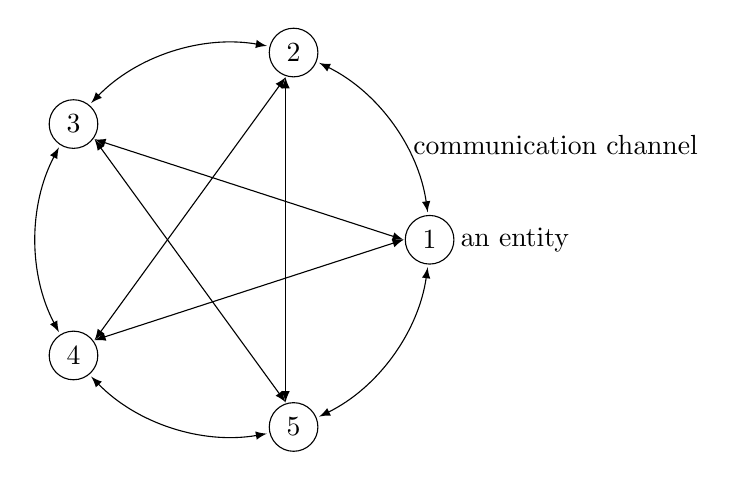
\begin{tikzpicture}

    \def \n {5}
    \def \radius {2.5cm}
    \def \margin {8} % margin in angles, depends on the radius
    % define coordinates for nodes
    \coordinate (A) at ({360/\n * (1 - 1)}:{\radius-3.3mm});
    \coordinate (B) at ({360/\n * (2 - 1)}:{\radius-3.3mm});
    \coordinate (C) at ({360/\n * (3 - 1)}:{\radius-3.3mm});
    \coordinate (D) at ({360/\n * (4 - 1)}:{\radius-3.3mm});
    \coordinate (E) at ({360/\n * (5 - 1)}:{\radius-3.3mm});
    
    % draw the circle
    \foreach \s in {1,...,\n}
    {
      \node[draw, circle] (\n) at ({360/\n * (\s - 1)}:\radius) {$\s$};
      \draw[<->, >=latex] ({360/\n * (\s - 1)+\margin}:\radius) 
      arc ({360/\n * (\s - 1)+\margin}:{360/\n * (\s)-\margin}:\radius);
    }
    % draw the mesh and labels
    \draw[<->, >=latex] (A) -- (C);
    \draw[<->, >=latex] (A) -- (D);
    \draw[<->, >=latex] (B) -- (D);
    \draw[<->, >=latex] (B) -- (E);
    \draw[<->, >=latex] (C) -- (E);
    \node at (A) [right=+6mm] {an entity};
    \node at (A) [above=+12mm,right] {communication channel};
  \end{tikzpicture}
  \caption{A possible event structure}
  \label{fig:structure}
\end{figure}

Figure~\ref{fig:structure} shows an example network of five nodes which
are all linked together. Each of the five nodes ($A..E$) can have some internal
and maybe observable state and messages are send over the communication channels
to the other entities of the network. 

The underlaying computational model for the entities or nodes is the
message automata. This follows the assumption that ``the universe is run by
computation''~\cite{bickford2005causal} and the everything can be modelled
by functionally updating the state and the message queues on the communication
channels of some entity. The proposed update function is $s':=f(s,v)$ where
the next state $s'$ follows from the current state $s$ and some internal or
external message $v$. $f$ is some arbitrary function which computes
the update step.~\cite{bickford2005causal}

To axiomatize these structure two types which are disjoint and two partial
functions are needed. The equality of the types are decidable.

\begin{defi}
  The large type of discrete types is
  $\mathcal{D}:=\{T:Type\ |\ \forall x,y:T.x=y\ in\ T\vee\neg (x=y\ in\ T)\}$.
  \textnormal{~\cite{bickford2005causal}}
\end{defi}

\begin{table}[h]
  \centering
  \begin{tabular}{l|l}
    Elements & Description\\\hline
    \textbf{E}$:\mathcal{D}$ & The type of possible discrete events.\\
    \textbf{Loc}$:\mathcal{D}$ & The type of possible discrete entities.\\
    \textbf{pred?}$:E\rightarrow (E+Loc)$
             & Return either the preceding event of\\
             & a location or the location itself.\\
    \textbf{sender?}$:E\rightarrow (E+Unit)$
             & Return the event which sents $e$ if e was sent or nothing.\\
  \end{tabular}
  \caption{The main types and functions for ordered event structures.~\cite{bickford2005causal}}
  \label{tab:eorder}
\end{table}

Table~\ref{tab:eorder} shows the signature of event structures with order.

From these functions we derive the next ones using the $is\_left$ which decides
on union types $(A+B)$ if the element is on the left side.
The function \[first(e)=\ if\ is\_left(pred?(e))\ then\ true\ else\ false\]
returns true if $e$ is the first event happening at some location.
The other function derived is $recv?(e)=\ if\ is\_left(sender?(e))\ then\ true\
else\ false$ returns true if the event $e$ was sent by another event.~\cite{bickford2005causal}

From these function we define the order relation.

\begin{defi}
  The strongly well-founded oder relation is
  $pred!(e,e') == (\neg first(e') \Rightarrow e = pred?(e')) \vee e = sender(e')$.
  This is the causal order relation from Lampert and denoted by $e<e'$.
\end{defi}

Additionally, there are three axioms that are needed to constraint the
event structure.~\cite{bickford2005causal}

\begin{axiom}
  If there is an event $e$ which triggers another event, then there is an
  event $e'$ such that for any event $e''$ which got triggered, $e''=e'$
  or $e''<e'$.
  \[\forall e:E.\exists e':E.\forall e'':E.(recv?(e'')\&sender?(e'')=e)\Rightarrow (e''=e'\vee e''<e)\]
\end{axiom}

\begin{axiom}
  The function $pred?$ is injective.
  \[\forall e,e':E.loc(e) = loc(e')\Rightarrow pred?(e) = pred?(e')\Rightarrow e=e'\]
\end{axiom}

\begin{axiom}
  The function $pred!$ is strongly well founded.
  \[\exists f:E\rightarrow \mathbb{N}.\forall e,e':E.pred!(e,e')\Rightarrow f(e)<f(e')\]
\end{axiom}

Axiom 3 can be explained as a ``tour'' through the event structure where
events happen as they're examined on the tour. This means that local
events are linearly ordered at each location and a recieve only happens
after a corresponding send.~\cite{bickford2005causal}

From that assumptions we define the finite list of events before a given event as
\[before(e):=\ if\ first(e)\ then\ []\ else\ pred?(e)\ append\ before((pred?(e)))\] 
and likewise the finite tree of all events causally before e as
\begin{align*}
  prior(e):= & if\ first(e)\ then\ []\ else\\
             & if\ recv?(e)\ then\ <e,prior(sender?(e)),prior(pred?(e))>\\
             & else\ <e,prior(pred?(e))>
\end{align*}

This basic language allows to describe event structures but to make
it more useful events should send values to each other. To distinguish
between internal events a discrete type called Act is used.~\cite{bickford2005causal}

\begin{defi}
  The type of an event is $kind :=\ Act + Top$ where $Act$ is some
  internal action and right some external one. The corresponding function
  $kind: E\rightarrow Act + Top$ returns the value of some event.
\end{defi}

\begin{defi}
  $Ty:Loc\rightarrow kinde\rightarrow Type$ returns the type of some event value at some specific
  node. For internal events $val:E\rightarrow Ty(loc(e),kind(e))$ can be any element of
  $Ty(e,a)$ choosen by any method.
\end{defi}





\begin{figure}
  \center
  \begin{tikzpicture}[node distance=2cm,auto,>=stealth]
    \node[] (server) {$B$};
    \node[left = of server] (client) {$A$};
    \node[below of=server, node distance=3cm] (server_ground) {};
    \node[below of=client, node distance=3cm] (client_ground) {};
    % vertical line
    \draw (client) -- (client_ground);
    \draw (server) -- (server_ground);
    % horizontal lines
    \draw[->] ($(client)!0.2!(client_ground)$) node[above,scale=0.5,left]{$a_1(3)$} -- ($(server)!0.3!(server_ground)$) node[above,scale=0.5,right] {$recv(3)$};
    \draw[<-] ($(client)!0.5!(client_ground)$) node[above,scale=0.5,left]{$recv(4)$} -- ($(server)!0.4!(server_ground)$) node[above,scale=0.5,right]{$b_1(4)$};
    \draw[->] ($(client)!0.6!(client_ground)$) node[below,scale=0.5,left]{$a_2(5)$} -- ($(server)!0.7!(server_ground)$) node[below,scale=0.5,right]{$recv(5)$};
    \draw[<-] ($(client)!0.9!(client_ground)$) node[below,scale=0.5,left]{$recv(6)$} -- ($(server)!0.8!(server_ground)$) node[below,scale=0.5,right]{$b_2(6)$};
  \end{tikzpicture}
  \label{fig:sequence}
  \caption{A message sequence diagram with an event structure between to
    processes A and B.}
\end{figure}

The figure~\ref{fig:sequence} shows a simple event structure between two
processes. The process $A$ sends a natural number to process $B$ which adds
one to the value and retuns the result.

To model the fact that an event $e$ can depend on a previous event $e'$ at
some location the notion of state and three relations are introduced.~\cite{bickford2005causal}

\begin{defi}
  $Identifiers$ $Id:\mathbb{D}$ are the discrte type of names of state variables where each
  holds a value with some specific type $T:x:Id\rightarrow i:Loc\rightarrow Type$.
\end{defi}

\begin{defi}
  For each location $i$ the state is the mapping of $Id\rightarrow T(x,i)$.
  The relations are \textbf{initially:} $x:Id\rightarrow i:Loc\rightarrow T(x,i)$,
  \textbf{when:} $x:Id\rightarrow e:E\rightarrow T(x,loc(e))$ and \textbf{after:} $x:Id\rightarrow e:E\rightarrow T(x,loc(e))$.
\end{defi}

\begin{axiom}
  The state of a value is for any event $e$ except the first, the value after
  the preceding event $e'$ where $e'<e$.
  \[\forall e:E.\neg first(e)\Rightarrow (x\ \textbf{when}\ e) = (x\ \textbf{after}\ pred(e))\]
\end{axiom}

The axiom refers to the fact that the value only changes after some event
happening. The change of the state is modeled as $\triangle$ operator with the
following definition.~\cite{bickford2005causal}

\begin{defi}
  The formula $x\triangle e = (x\ \textbf{after}\ e\ne x\ \textbf{when} e)$ returns true
  if some event $e$ changes the state variable $x$.
\end{defi}

\begin{defi}
  The formula $\triangle (x,e) = ||[e_1\in \textbf{before}(e)|x\triangle e_1]||$ is only defined when
  $T(loc(e),x)$ has decidable equality and true if there are exactly $n$ changes to
  exactly $x$ before the event $e$ happens.  
\end{defi}

\begin{defi}
  The formula $x\triangle_n e = 0<n\wedge \triangle (x,e)=n-1\wedge x\triangle e$ returns true if there are
  exactly $n$ changes unit $x$ and including the event $e$.
\end{defi}

The communiction between locations is modeled as a link or communication
channel as mentioned earlier. To abstract away specific topologies the structure
is imagened as directed graph between the nodes or locations.~\cite{bickford2005causal}

\begin{defi}
  A link between a source and destination is a labeled pair $l=<i,j>$.
  \textbf{Link:} $\mathbb{D}$ is the discrete type of links.\\
  \textbf{src:} $Link\rightarrow Loc$ and \textbf{dst:} $Link\rightarrow Loc$ returns the sender
  or reciever of a message.
\end{defi}

A link can send multiple messages $m$ of $Type\ T$ over a link.
In order to distinguish between the messages a discrete type $Tag$
is added to the messages on the link and processed in first-in-first-out order.~\cite{bickford2005causal}

\begin{defi}
  the function $M:Link\rightarrow Tag\rightarrow Type$ types a tagged message on a link.
\end{defi}

\begin{axiom}
  The processing happens in first in first out order.\\
  $\forall e_1,e_2:E.recv(l,t)(e_1)\ \&\ recv(l,t)(e_2) \Rightarrow sender?(e_1)<sender?(e_2)\Rightarrow e_1<e_2$
\end{axiom}

So far, the language specification of event structures consists out of events
which send messages over links to different or the same node and trigger new
events based on some update function and the nodes state. In addition, time
is needed to reason about realtime properties and changes over time.~\cite{bickford2005causal}

\begin{defi}
  Time is a map $time:E\rightarrow Time$ added to the event structure where $Time$
  is the rational numbers. The time of events is also ordered $e_1\prec e_2\Rightarrow
  time(e_1)\le time(e_2)$.
\end{defi}

\begin{defi}
  State changes are modeled as step function which implicitly depending on time.
  $discrete:Id\rightarrow Id\rightarrow \mathbb{B}$ such that a varaible $x$ can only be changed
  from one constant to another.
\end{defi}

\begin{axiom}
  $\neg first(e)\Rightarrow \forall t\ge 0.(x\ \textbf{when}\ e)(t)=
  (x\ \textbf{after}\ pred(e))(t+time(pred(e))-time(e))$
\end{axiom}

\paragraph{Computing Model}

% nachrichtenautomat
Grundlage für die Eventlogik ist ein Nachrichtenautomat. Dieser ist ein
nichtdeterministischer Automat der auf Nachrichten operiert.
Er hat die drei Basisoperationen ``senden'', ``empfangen'' und ``interne
Zustandsänderung''.~\cite{bickford2003logic}

\begin{defi}
  Ein Event $e=(a+m)$ ist ein Typ $A+M$ der entweder eine interne Aktion $A$ enthält
  oder eine empfangene Nachrichten $M$.
\end{defi}

\begin{defi}
  Ein Nachrichtenautomat ist ein abhängiger Datentyp mit der Struktur:
  $\{St, Act, Msg: Type, init: St$
    $f:(Act+Msg)\rightarrow St\rightarrow St$
    $send:(Act+Msg)\rightarrow St\rightarrow MsgList\}$
\end{defi}

% verteilte Nachrichtenautomaten
Um verteilte Systeme darstellen zu können wird mehr als ein Nachrichtenautomat
benötigt, da ein Nachrichtenautomatenohne Interaktionen ein normaler
nichtdeterministischer Automat ist. Ein verteiltes System $V$ ist eine Menge von
Nachrichtenautomaten die in einem Netzwerk miteinander verknüpft sind.
Das Netzwerk ist fair, d.h. jede gesendete Nachricht wird auch unverändert
empfangen.~\cite{bickford2003logic}

\begin{defi}
  Ein verteiltes System $V$ ist ein Tupel $V=(M,L)$ wobei $m_i\in M$ mit $i\in
  \mathbb{N}$ die Menge der teilnehmenden Nachritenautomaten ist. $L$ beschreibt
  ein Kante in einem gerichteten Graphen und besteht aus dem Tupel $L=(s,d,m_i,m_j,Q)$
  mit $i,j\in \mathbb{N} und i!= j.Q$ ist eine Nachrichtenqueue.
\end{defi}

\subsection{COQ}

%%% Local Variables:
%%% mode: latex
%%% TeX-master: "../master"
%%% End:
